\section{Commenti dati USTAT}
Per inquadrare il nuovo comune nato dalla fusione di realtà diverse, abbiamo ritenuto opportuno proporre un’analisi quantitativa della popolazione e dell’occupazione 
Questo approccio  è necessario se si vuol parlare di riqualifica urbana in quanto permette di conoscere con accuratezzale dinamiche e la particolarità dei diversi quartieri, all’interno della nuova realtà comunale. Capire deve sono i luoghi di lavoro e dove invece quelli residenziali, permette poi di pianificare la nuova città, creando le interconnessione necessarie per migliorare la qualità di vita delle persone

\subsection{Analisi demografica}
Attraverso un’analisi dell’evoluzione della popolazione dal 1990 fino al censimento più recente del 2016 si è arrivati a diverse conclusioni. L’incremento maggiore è stato registrato  nei comuni di Claro, Monte Carasso, Gnosca e Gudo; raggiungendo una variazione attorno al 70\%.  Mentre al centro (Bellinzona e Giubiasco) la crescita è stata poco rilevante. In questi 27 anni, la popolazione ha emigrato verso le zone periferiche della città dove i costi degli immobili sono inferiori ma, forse, alla ricerca di calma e tranquillità. Queste dinamiche comportano però spostamenti quotidiani dal luogo di residenza a quello lavorativo nel coso i due luoghi non coincidono come nel nostro caso (confronto tra tab. 1 e 2) . L’utilizzo della vettura privata per spostarsi concentra il traffico nelle ore di inizio e fine lavoro. La creazione di una via intelligente e alternativa destinata alla mobilità lenta è necessaria (assieme naturalmente all’ampliamento dei servizi pubblici). Con la realizzazione di una vera propria rete di piste ciclabili che collegano la periferia al centro di Bellinzona.

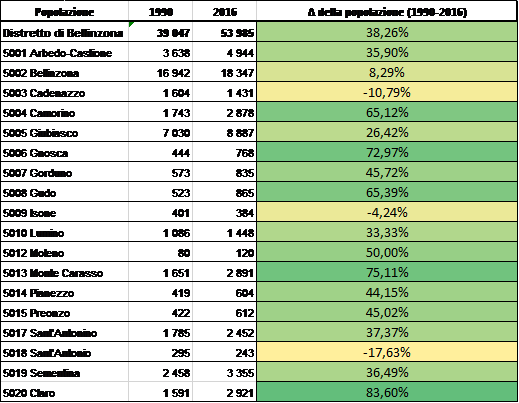
\includegraphics[scale=0.5]{Capitoli/immagine progetto.png}

\subsection{Analisi economica}
Per analizzare il nuovo comune sotto l’aspetto economico, si possono prendere i dati dell’ufficio cantonale di statistica che riguardano i lavoratori a tempo pieno. Si può notare una variazione importante nei comuni di Arbedo – Castione (62,5\%) (che non fa però parte del nuovo comune) e nei due piccoli comuni di Moleno e Sant’Antonio (ma i valori in termini assoluti sono irrilevanti). Mentre dove l’impiego è aumentato in maniera considerevole sono i comuni di Monte Carasso (588 posti di lavoro a tempo pieno, +34,4\%), Cadenazzo (1404, +18.9\%), Sementina (795, +17,6\%), Tuttavia la maggior poste dei posti di lavoro sono concentrati a Bellinzona (53\%) e, in minor misura, Giubiasco (12\%). Inoltre, solo una piccola minoranza ha la possibilità di lavorare nel luogo dove risiede e questo comporta continui spostamenti giornalieri.  
\\
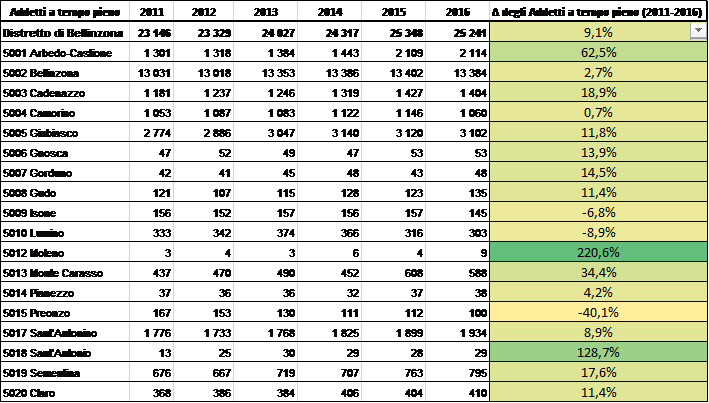
\includegraphics[scale=0.5]{Capitoli/ioioi.png}
\\Un confronto possibile è il rapporto abitante – posto di lavoro del distretto di Bellinzona in confronto con la percentuale Cantonale e quella Nazionale.

----TABELLA---
\\
La città di Bellinzona si trova al di sopra della media Svizzera, grazie ai numerosi uffici amministrativi cantonali, mentre il distretto di Bellinzona ha un rapporto inferiore in quanto all’interno del distretto vi sono dei quartieri nella quale sono perlopiù residenziali e quindi non offrono un impiego. Attenzione: città o quartiere, distretto o città?

\subsection{Conclusione}
Questa breve analisi evidenzia un problema comune a tutte le città: nei centri ci sono la maggior parte dei posti di lavoro mentre la popolazione tende a spostarsi nelle periferie dove i costi dell’alloggio sono inferiori. La contropartita a questa evoluzione è naturalmente un incremento del traffico. Nel caso specifico di Bellinzona il problema è poi amplificato dal traffico proveniente da fuori, legato ai numerosi posti di lavoro nella Pubblica amministrazione. Limitandoci alla popolazione urbana, è però possibile contenere il problema incrementando la mobilità lenta con piste ciclabili efficaci.
Anche perché su percorsi brevi (attorno ai 5-8 km) la biciletta ha tempi di percorrenza inferiori a quella dell’auto negli orari di punta, naturalmente a condizione che esistano delle piste ciclabili adeguate. Naturalmente anche i mezzi pubblici possono essere efficaci, ma richiedono più investimenti e interventi importanti per renderli competitivi.
Nel seguito del nostro lavoro, ci concentreremo soprattutto sulle piste ciclabili, perché possono ridurre il traffico veicolare ma soprattutto perché potrebbero essere un ottimo strumento di connessione e legame tra i vari quartieri.

---TABELLAA---

